% Pour commencer, nous avons généré des nombres aléatoires avec la bibliothèque \texttt{random} de python sans les convertir en nombres décimales et nous les avons testés avec tout les différents test implémenté plus haut. En faisant cela, nous avons remarque que les résultats obtenus pour nos hypothèses $H_0$ et $H_1$ étaient presque similaire à ceux que nous avions lorsque nous testions notre générateur.  

Pour la comparaison de notre générateur contre le générateur par défaut de Python. Pour ce faire, nous avons, pour les deux générateurs, lancer la génération de n nombres et tester ces nombres avec nos tests, et faire cela k fois. Avec cela, nous avons pu déterminer  la p-valeur moyenne pour chaque test. la reussite global du test de Gap s'explique par le fait que dans par sont fonctionnement puisque pour appliquer notre test :
\begin{itemize}
    \item on normalise notre séquence par son maximun dans le cas ou les nombres de la séquence ne sont pas compris entre 0et 1
    \item puis on teste la  séquence ainsi normalisée
\end{itemize}
    cela a pour but de ne pas avoir à redefinir l'intervalle $[a,b[$ et le paramètre $p = b-a $   de la loi géométrique


    les résultats numériques obtenu pour :


    \newpage

\begin{itemize}
     
    \item pour  k = 10 , n = 100.000
        \begin{center}

            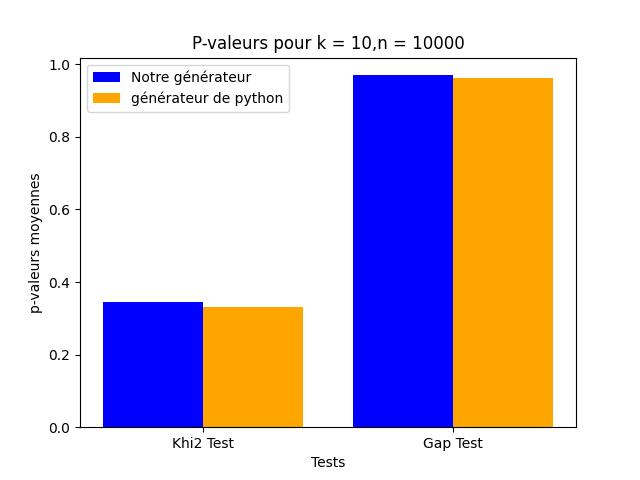
\includegraphics[width=0.5\linewidth]{rapport//images//fig/figk10n100000.jpg}
            \caption{Enter Caption}
            \label{fig:enter-label}
   
            \begin{tabular}{c|c|c}
                \hline
                Tests & p-valeur moyenne & taux de reussite \\
                \hline
                    \multicolumn{3}{c}{Notre generateur} \\
                \hline
                $\chi^2$ & 0.346  & 70\% \\
                
                Gap & 0.970 &  100 \%\\
                \hline
                 \multicolumn{3}{c}{generateur python} \\
                \hline
                $\chi^2$ & 0.331 & 90\% \\
                
                Gap & 0.961 & 100\%\\
                \hline
            \end{tabular}
        \end{center}
        
    \item  (k = 100 , n = 100.000 ) 
         \begin{center}
    
            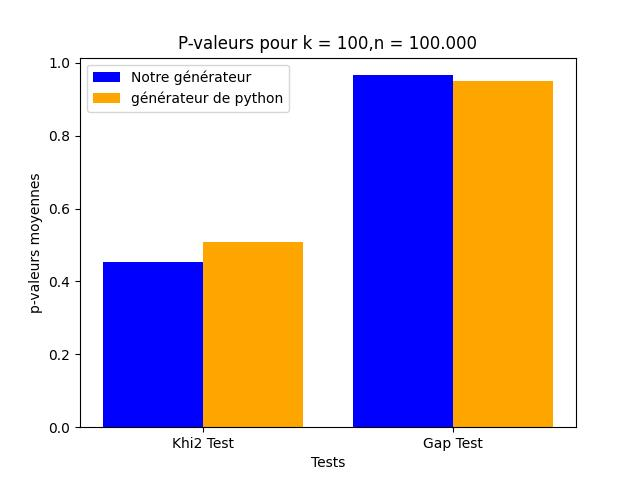
\includegraphics[width=0.5\linewidth]{rapport//images//fig/figk100n100000.jpg}
            \caption{Enter Caption}
            \label{fig:enter-label}
               
            \begin{tabular}{c|c|c}
                \hline
                Tests & p-valeur moyenne & taux de reussite \\
                \hline
                    \multicolumn{3}{c}{Notre generateur} \\
                \hline
                $\chi^2$ & 0.453  & 88\% \\
                
                Gap & 0.966 &  100 \%\\
                \hline
                 \multicolumn{3}{c}{generateur python} \\
                \hline
                $\chi^2$ & 0.508 & 90\% \\
                
                Gap & 0.951 & 100\%\\
                \hline
            \end{tabular}
            
       \end{center}
    
    \item (k = 100 , n = 500.000 ) 
       \begin{center}

            \begin{tabular}{c|c|c}
                \hline
                Tests & p-valeur moyenne & taux de reussite \\
                \hline
                    \multicolumn{3}{c}{Notre generateur} \\
                \hline
                $\chi^2$ & 0.316  & 89\% \\
                
                Gap & 0.899 &  100 \%\\
                \hline
                 \multicolumn{3}{c}{generateur python} \\
                \hline
                $\chi^2$ & 0.495 & 95\% \\
                
                Gap & 0.918 & 100\%\\
                \hline
            \end{tabular}
       \end{center}
    


   \item  (k = 100 , n = 100.000 ) 
       \begin{center}
            \begin{tabular}{c|c|c}
                \hline
                Tests & p-valeur moyenne & taux de reussite \\
                \hline
                    \multicolumn{3}{c}{Notre generateur} \\
                \hline
                $\chi^2$ & 0.453  & 88\% \\
                
                Gap & 0.966 &  100 \%\\
                \hline
                 \multicolumn{3}{c}{generateur python} \\
                \hline
                $\chi^2$ & 0.508 & 90\% \\
                
                Gap & 0.951 & 100\%\\
                \hline
            \end{tabular}
       
        \end{center}
\end{itemize}



    Nous pouvons observer que le générateur Python garde une certaine constance pour les p valeur moyenne pour le test de $\chi^2$1, contrairement à notre générateur dont les p-valeur décroissent grandement avec lorsque le nombre n de nombre générés augmente

    par contre pour le test de Gap , la p-valeur reste cmoyennement constante quelqu'en
    soit le générateur 